\subsection{Para onde vai um conteúdo reprovado?}

\textbf{Cena 3, Abril de 2017.\footnote{Cena escrita a partir de entrevista realizada com Alberto Lima no Rio de Janeiro, no dia 06 de fevereiro de 2020. Quando não explicitamente atribuídas a outrem, todas as aspas desta sessão são falas do entrevistado.} Rio de Janeiro.}

O engenheiro Alberto Lima, professor do curso técnico em Eletrônica do CEFET/RJ, liga seu computador decidido a criar o verbete ``Andes-SN'' na Wikipédia, para falar sobre o Sindicato Nacional dos Docentes das Instituições de Ensino Superior.

Concursado em 2011, Alberto participou ativamente do movimento grevista de 2012, greve esta deflagrada pelas bases em assembleia, contrariando indicação das direções sindicais. Após integrar o comando local de greve, inclusive participando de grandes atos em Brasília/DF, Alberto se junta a companheiros/as paredistas em 2013, concorre, e ganha a eleição para a direção da Adcefet-rj, seção sindical do Andes em sua instituição.

Ao final de sua gestão como presidente do sindicato local, em 2017, Alberto acreditava que o Andes-SN, apesar de ser um dos maiores sindicatos do Brasil, com seções em todas as universidades federais, não possuía uma grande presença digital. Resolveu ler sobre boas práticas de criação de verbetes na Wikipédia e, apesar da dica encontrada de começar editando artigos pré-existentes ao invés de criar um novo do zero, sentiu-se preparado para criar um verbete. Pesquisou se existiam artigos sobre outras entidades similares à sua, e se lembra de ter encontrado vários, ``\textit{alguns inclusive bem curtos com apenas uma referência}''. Com sua pesquisa feita, sentiu-se confiante e começou a escrever sobre seu sindicato nacional.

O professor nos conta que começou a escrever direto na página da Wikipédia. Fez um texto longo, ``\textit{que tinha inclusive uma ligação interna}'', duas referências e estruturado com ``\textit{Introdução} e "\textit{contextualização}''. Se sentia seguro e confortável ao escrever alí, pois afinal ``\textit{qualquer um pode editar a Wikipédia}''.
	
Sabia que seu texto ``\textit{não estava completamente redondo}'', mas resolveu salvar como estava para continuar mais tarde. Nosso editor novato nos conta que já tinha visto alguns verbetes na Wikipédia marcados com avisos como ``\textit{esboços}'', ``\textit{demandando estruturação}'' ou ``\textit{carece de referências}'', e sabia que a mesma coisa poderia acontecer com seu verbete, que seria melhorado mais tarde.

Porém, alguns segundos depois ele é surpreendido por uma notificação informando que seu artigo havia sido removido pelo administrador EVinente, atendendo a um pedido de outro usuário. Ao acessar o endereço da página, se deparou com a seguinte imagem:

\begin{figure}[H]
    \centering
    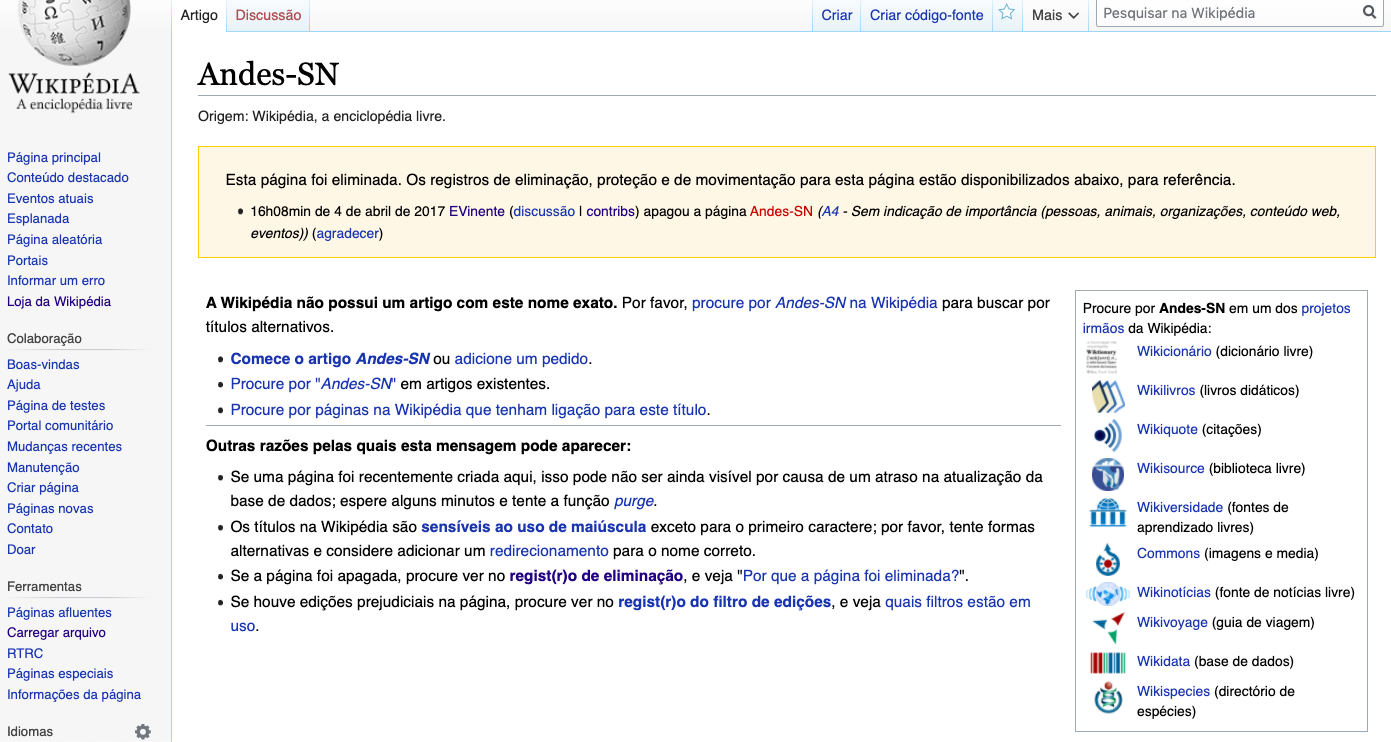
\includegraphics[width=1\textwidth]{Images/andes.png}
    \caption{Verbete Andes-SN com aviso de eliminação.}
    \label{fig:verbete_andes}
\end{figure}

Lembrando das apresentações assistidas nos seminários de pesquisa sobre controvérsias na Wikipédia, Alberto vai à página de discussão do usuário que solicitou a eliminação, onde o profesor então explica saber que o verbete ainda não estava ideal, que teria mais referências para adicionar (``\textit{notícia de greve é o que mais tem}''), inclusive com uma tese acadêmica sobre a história do sindicato. Concluiu informando que gostaria de continuar editando.

\begin{figure}[H]
    \centering
    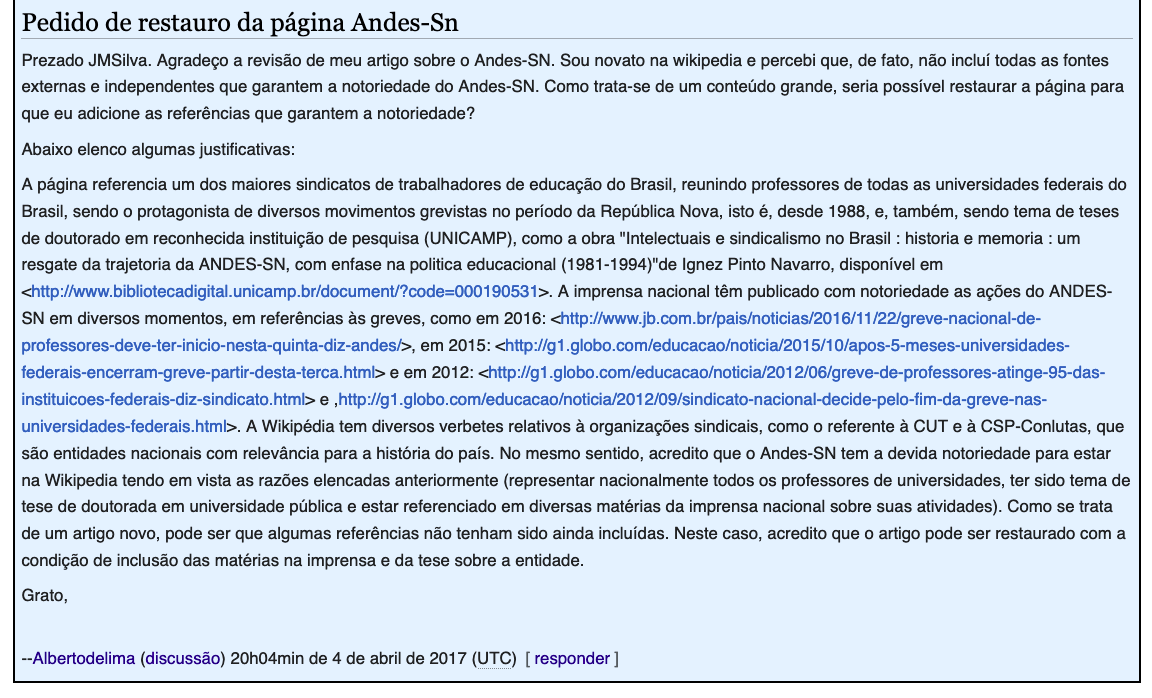
\includegraphics[width=1\textwidth]{Images/alberto-pedido-restauro.png}
    \caption{Página "Wikipédia:Pedidos/Restauro" com o pedido de Albertodelima para que a solicitação remoção feita por JMSilva fosse revista.}
    \label{fig:verbete_andes}
\end{figure}


O Diálogo então, segundo a memória de nosso protagonista, seguiu mais ou menos assim:

-Se você já sabia onde encontrar mais referências por que não as colocou logo?

-Eu estava sem tempo, mas vou colocar. Porém, o que eu já escrevi sumiu. Quero editar e melhorar, mas não tenho backup.

- Você vai ter que escrever tudo de novo.

Alberto, traído pela confiança na ferramenta, não seguiu sua prática corriqueira de escrever offline e depois "copiar e colar" o conteúdo criado em uma ferramenta online, e agora se via sem possibilidade de acessar novamente sua criação, eliminada do histórico público da Wikipédia.
Como resultado, ele, que estava ocupado com a reta final de seu mandato à frente da Adcefet-rj e já cursando doutorado, resolveu abrir mão de disputar a construção de conteúdos na Wikipédia. ``\textit{Eu nunca mais criei nenhum outro artigo. Nem esse.}''

No início de 2020, Alberto ficou feliz em ver que fora criado em 2018 outro verbete sobre o Andes-SN, desta vez levando seu nome completo, ``Sindicato Nacional dos Docentes das Instituições de Ensino Superior''. Apesar do novo verbete ser muito inspirado na seção ``Sobre'' da página sindicato, não apresentar nenhuma referência, ser muito menos acadêmico que o anterior, e de ter recebido as marcações de ``\textit{Este artigo não cita fontes confiáveis e independentes}'' e ``\textit{Este artigo é um esboço}'', em nenhum momento foi ``proposto para eliminação''.